\chapter{The Slip}

\vspace{1em}
\hfill
\begin{minipage}[c]{0.55\textwidth}
\raggedleft
\small\itshape
It from bit. Every it derives its function, its meaning, its very existence from the apparatus-elicited answers to yes-or-no questions.\\[0.5em]
\upshape\footnotesize John Archibald Wheeler, ``Information, Physics, Quantum'' (1990)
\end{minipage}%
\hspace{0.5em}
\begin{minipage}[c]{0.12\textwidth}
% \includegraphics[width=\textwidth]{figures/ch06_slip.png}
\end{minipage}
\vspace{1.5em}

\noindent \textsc{Chapter 5 ended with a small phrase.} \emph{What remains is interpretation.} This chapter examines the first step the mathematics does not force.

So far, the universal semimeasure $M$ has weighted candidate programs whose outputs begin with the data you have. It is a prior for sequential prediction.

The temptation is to read $M$ differently. Not as a measure over candidate descriptions, but as a measure over what is.

\section*{Two readings}

The equation $M(x) = \sum_{p\,:\,U(p) = x*} 2^{-|p|}$ does not say what $M(x)$ \emph{means}. It says how to compute it. Two interpretations are available, and they are not the same thing.

The first reading is epistemic. $M(x)$ is the weight assigned to seeing a prefix $x$ before further data. The universal construction tells you how to weight candidate programs. Nothing in this reading commits to anything about the world itself.

The second reading is ontic. It proposes that programs describe realities and that $M(x)$ somehow measures the realities producing $x$. But that ``somehow'' contains extra work. The formula weights programs and output prefixes. It does not tell us which outputs exist, how many observer occurrences an output contains, or how program weight should become ontic weight.

The mathematics is the same. The metaphysical commitment is different.

\begin{figure}[h]
\centering
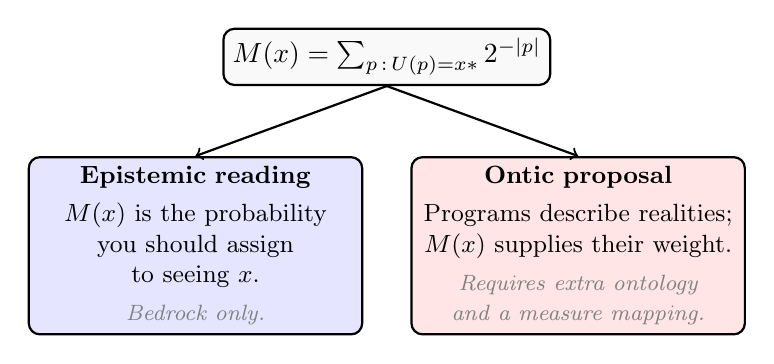
\begin{tikzpicture}[scale=0.9]
  % Top: the equation
  \node[draw, thick, rounded corners, fill=gray!5, font=\normalsize] (top) at (5, 5) {$M(x) = \sum_{p\,:\,U(p) = x*} 2^{-|p|}$};

  % Left box: epistemic
  \node[draw, thick, fill=blue!10, rounded corners, font=\small, text width=4cm, align=center, anchor=north] (left) at (2.3, 3.6) {\textbf{Epistemic reading} \\[0.3em] $M(x)$ is the probability \\you should assign \\to seeing $x$. \\[0.3em] \footnotesize\itshape\textcolor{gray}{Bedrock only.}};

  % Right box: ontic
  \node[draw, thick, fill=red!10, rounded corners, font=\small, text width=4cm, align=center, anchor=north] (right) at (7.7, 3.6) {\textbf{Ontic proposal} \\[0.3em] Programs describe realities; \\$M(x)$ supplies their weight. \\[0.3em] \footnotesize\itshape\textcolor{gray}{Requires extra ontology and a measure mapping.}};

  % Arrows
  \draw[->, thick] (top.south) -- (left.north);
  \draw[->, thick] (top.south) -- (right.north);
\end{tikzpicture}
\caption{The slip. The epistemic use is defined by the construction in Part I. The ontic proposal adds two claims the equation does not contain: which outputs exist and why program weights should measure them. The postulate below addresses privileged cuts; it does not supply an observer-occurrence measure.}
\label{fig:slip}
\end{figure}

This chapter exposes the second reading without quietly installing it. The next section labels the commitment the book does make.

\section*{The one move: no cut is privileged}

To deny that one decomposition is uniquely correct takes one step. Naming it precisely is the work of this chapter, because once it is named you can see its reach and refuse it.

Start with the language. The original Church-Turing thesis concerns what counts as an effective procedure. A stronger \emph{physical} Church-Turing thesis says that physically realizable processes can be simulated by Turing computation. That stronger claim is not a theorem of computer science, and physics has not closed it. This book therefore uses computable descriptions as its chosen frame. The frame is broad enough to express the theories used here, but choosing it neither proves that nature is computable nor says which descriptions are real.

Now the step itself. ``There is one world, decomposed in exactly this way'' is not a neutral description. It selects a system and a boundary. The postulate declines to call that decomposition view-independently correct.

\begin{quote}
\textbf{The postulate: no cut is privileged.} No decomposition of the describable totality is view-independently correct. Every carving into worlds, systems, and selves is a cut an observer makes; none comes labeled as the structure's own.
\end{quote}

This is the book's one interpretive commitment, and it is a refusal, not an addition. It does not announce that all computable structures exist. Under Picture A, one may contemplate the totality of descriptions as an object. Under Picture B, a situated observer retains a posterior over candidate descriptions. The postulate does not choose which picture is real.

Be careful how far this reaches. ``No cut is privileged'' is not ``every structure is equally, robustly real.'' The leap from declining to privilege one world to asserting that all of them exist in the full-blooded sense is \emph{itself} a cut, and the book does not make it either. Whether the totality ``exists'' is a question the book holds open; Chapter 8 shows why it has no view-independent answer. For now the commitment is only the refusal: no carving is the true one.

What the postulate buys is underdetermination. Many structures are consistent with partial data, and no decomposition arrives already crowned. Finitude explains why an observer must use bounded local models. The fair-bit construction, Kraft, dominance, and convergence explain why $M$ is a powerful ideal predictor. None of those claims makes simplicity the world's preference.

What the postulate costs is groundlessness. It withholds a view-independent answer to which decomposition is the real one. Picture A makes the cost vivid by contemplating many alternatives; Picture B keeps the uncertainty situated. The next section explains why the language of information tempts us toward Picture A, and why that temptation is not proof.

\section*{Information is in the cut}

A standard objection to Picture A is the one Occam's razor is usually summoned for: it multiplies entities. If every computable output is taken as a reality, the ontology is far larger than the single universe we observe.\footnote{A nearby position in the literature is Tegmark's Mathematical Universe Hypothesis, here restricted to computable structures. This book does not adopt it as a consequence of Solomonoff induction.} Occam's razor seems to forbid such inflation. \emph{Do not multiply entities beyond necessity.}

The objection rests on a confusion the Library makes visible.

Chapter 2 established that informational cost lives in the cut, not in the totality. The empty set is cheap. The universal set is cheap. Both are describable in a phrase. The interesting subsets, the ones that require selecting some elements from a larger possibility space, are where description length lives.

Apply the principle to ontology. Two competing positions on what exists.

\begin{figure}[h]
\centering
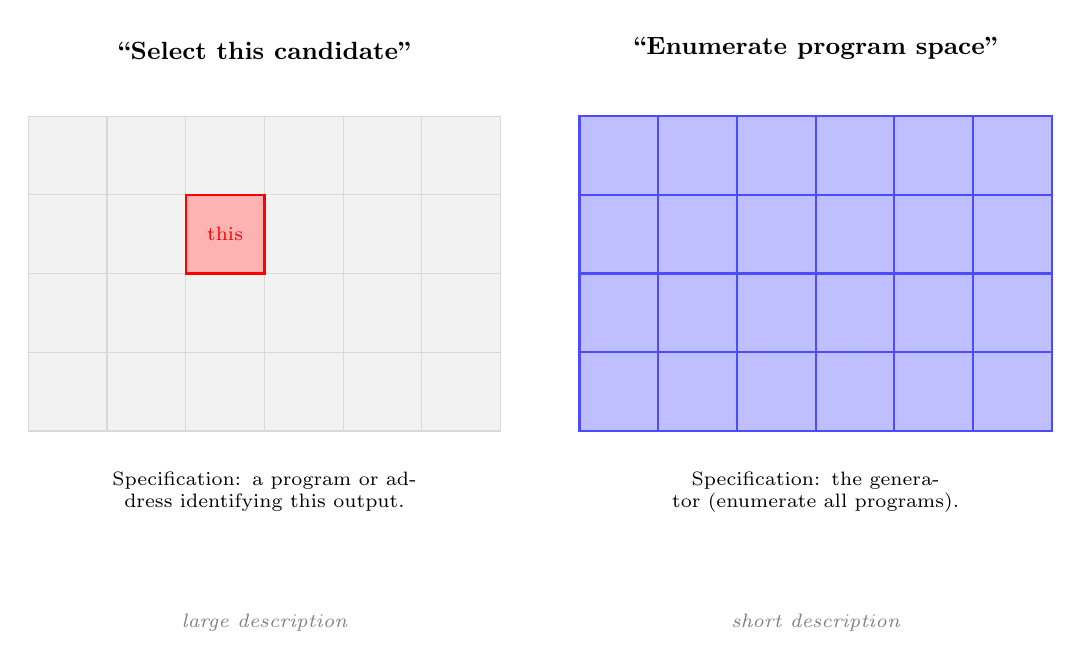
\begin{tikzpicture}
  % LEFT: Select one candidate
  \node[font=\small\bfseries, anchor=south] at (3, 4.6) {``Select this candidate''};

  % Faded grid of universes (Library, mostly grayed)
  \foreach \x in {0,1,2,3,4,5} {
    \foreach \y in {0,1,2,3} {
      \draw[gray!30, fill=gray!10] (\x, \y) rectangle ({\x+1}, {\y+1});
    }
  }
  % One highlighted universe
  \draw[thick, red, fill=red!30] (2, 2) rectangle (3, 3);
  \node[font=\scriptsize, red] at (2.5, 2.5) {this};

  % Label below
  \node[font=\scriptsize, anchor=north, text width=5.5cm, align=center] at (3, -0.4) {Specification: a program or address identifying this output.};
  \node[font=\scriptsize\itshape, anchor=north, gray] at (3, -2.2) {large description};

  % RIGHT: Enumerate program space
  \node[font=\small\bfseries, anchor=south] at (10, 4.6) {``Enumerate program space''};

  % Fully lit grid
  \foreach \x in {7,8,9,10,11,12} {
    \foreach \y in {0,1,2,3} {
      \draw[thick, blue!70, fill=blue!25] (\x, \y) rectangle ({\x+1}, {\y+1});
    }
  }

  % Label below
  \node[font=\scriptsize, anchor=north, text width=5.5cm, align=center] at (10, -0.4) {Specification: the generator (enumerate all programs).};
  \node[font=\scriptsize\itshape, anchor=north, gray] at (10, -2.2) {short description};
\end{tikzpicture}
\caption{Two descriptions side by side. Selecting one candidate (left) requires information that identifies it. Describing the whole program space (right) requires only an enumerator. This compares code lengths in a chosen language; it does not establish which ontology is true.}
\label{fig:cut-argument}
\end{figure}

\emph{Description One: select this candidate.} Within the Library metaphor, identifying a particular complete output requires a program or address. Its cost is relative to the chosen machine. We do not know the Kolmogorov complexity of our universe, and a metaphysical claim is not literally a codeword, but selection carries descriptive information that ``enumerate all'' does not.

\emph{Description Two: enumerate every program.} An enumerator can be written compactly: \emph{dovetail all programs and record their outputs}.\footnote{``Generator'' is metaphor. Program space is a mathematical object; the pseudocode is our compact description of it, not evidence that a cosmic computer runs it in time.} Its description is short on ordinary reference machines.

As descriptions, ``enumerate all'' can be shorter than ``select this exact member.'' That is an observation about code length, not a theorem that the larger ontology is true or probable.

This does not prove the postulate. Applying description length to existence is a further step, and the comparison depends on the language in which the positions are encoded. It does reframe one intuition: an unrestricted generator may have a shorter description than an exact selection. Ontological parsimony and program length are not automatically the same thing.

The book takes the postulate because it refuses a view-independent decomposition. The compactness of the generator motivates the picture but does not establish it.

\section*{Where this leaves you}

The slip has been exposed. The universal semimeasure weights candidate programs and prefixes. Reading it as a measure on realities requires additional ontology, and reading it as a measure over observer occurrences requires more again. The postulate denies privileged cuts without supplying either measure.

The two pictures this leaves open, the older question they sharpen, and their limits are the subjects of the next chapter.
